\documentclass[11pt,a4paper,twoside,pdf]{article}

% Paquetes (añade otros si los necesitas):
\usepackage{latexsym}
\usepackage[utf8x]{inputenc}
\usepackage{soul}
\usepackage{array}
\usepackage{amsmath}
\usepackage{amssymb}
\usepackage{marvosym}
\usepackage{epsfig}
\usepackage{graphics}
\usepackage{amsfonts}
\usepackage{xspace}
\usepackage{color}
\usepackage{booktabs}
\usepackage{xtab}
\usepackage[colorlinks=true,urlcolor=blue,linkcolor=blue,citecolor=blue]{hyperref}
\numberwithin{equation}{section}

% Fuente: palatino
\usepackage[sc]{mathpazo}
\linespread{1.05}

% TFG en inglés:
%\usepackage[english]{babel} 
%\addto\captionsenglish{\renewcommand{\chaptername}{}}

% TFG en español:
\usepackage[spanish,es-nodecimaldot,es-tabla,es-lcroman,es-nosectiondot,
            es-noindentfirst]{babel}
\renewcommand\spanishchaptername{}

% Formato de la página:
\usepackage{fancyhdr}
\usepackage[top=2.88cm,bottom=2.97cm,left=2.95cm,right=2.95cm]{geometry}
\setlength{\parskip}{0.1cm}

% Pon aquí tus definiciones:

\newcommand{\dis}{\displaystyle}
\sodef\an{}{.2em}{1em plus1em}{2em plus.1em minus.1em}

\begin{document}

% Portada %%%%%%%%%%%%%%%%%%%%%%%%%%%%%%%%%%%%%%%%%%%%%%%%%%%%%%%%%%%%%%%%%%%%%%

\pagestyle{empty}


\noindent
\begin{tabular}{r}

\includegraphics[width=8.8cm]{escudoUGRmonocromo.png} \\[-1.8ex]
\hspace{31mm}\vspace{-8mm}
\begin{tabular}{c}
\hline\\[-1ex]\hskip-2mm
{\bf Facultad de Ciencias}\hspace{18mm}
\end{tabular}
\end{tabular}

{\large
\vspace{30mm}
\hspace{25mm}
\begin{tabular}{l}
\an{GRADO EN FISICA}
\end{tabular}

\vspace{45mm}
\hspace{25mm}
\begin{tabular}{l}
\an{TRABAJO FIN DE GRADO}
\\[1.5ex]
\an{\LARGE\bf IMPLEMENTACI\'ON DE }
\\
\an{\LARGE\bf M\'ETODOS}
\\
\an{\LARGE\bf EN DIFERENCIAS FINITAS }
\\
\an{\LARGE\bf EN GPUs}
\end{tabular}

\vfill
\hspace{25mm}
\begin{tabular}{l}
Presentado por:
\\
{\bf D. JUAN JOS\'E SALAZAR L\'OPEZ}
\\[3ex]
Curso Académico 2021/2022
\end{tabular}
}


\newpage

\begin{center}

{\bf Resumen}
\bigskip

\begin{minipage}{0.8\linewidth}
El método numérico de las diferencias finitas dependientes del tiempo (FDTD) se usa como herramienta para la resolución de ecuaciones diferenciales de primer orden.  Este cobra especial importancia en la electrodinámica computacional dado que nos permite resolver las ecuaciones de Maxwell realizando algoritmos con los que calcular punto a punto los valores del campo electromagnético. Estos algoritmos se implementan generalmente usando la potencia de cálculo que nos proporcionan las CPUs y dada la necesidad de discretizar el espacio, el timepo empleado en el proceso de cálculo aumenta con las dimensiones del problema. En este TFG se han generado varios algoritmos de uso libre en CUDA para exponer las ventajas que se obtienen al implementar este método usando el poder de paralelización que nos proporcionan las GPUs, lo que disminuye el tiempo empleado en el cálculo de los campos. 
\end{minipage}

\vfill

{\bf Abstract} 
\bigskip

\begin{minipage}{0.8\linewidth}
The numerical method of the finite differences time domain (FDTD) is used to solve once order differential equations. This method is specially useful in the computational electrodynamics since we can solve Maxwell equations using algorithms to calculate the electromagnetic field point to point. These algorithms are usually implemented using the calculus power of CPUs and, due to the need to discretyze space, the calculate time increase with the problem size. In this TFG it has been developed some CUDA open source algorithms to show the parallelization power given by the GPUs, which allows us to decrease the time needed to calculate the fields.
\end{minipage}

\vfill

\end{center}

% Indice %%%%%%%%%%%%%%%%%%%%%%%%%%%%%%%%%%%%%%%%%%%%%%%%%%%%%%%%%%%%%%%%%%%%%%%
\newpage

\tableofcontents

% Texto %%%%%%%%%%%%%%%%%%%%%%%%%%%%%%%%%%%%%%%%%%%%%%%%%%%%%%%%%%%%%%%%%%%%%%%%
\newpage

\pagestyle{fancy}
\fancyhead[RO,LE]{\leftmark}
\fancyhead[LO,RE]{\thepage}
\fancyfoot{}

\section{Introducción}
El método numérico de las diferencias finitas es usado en muchos campos para la resolución de ecuaciones diferenciales de primer orden \cite{Taflove2005}. En particular, el método de la diferencia central finita cobra especial importancia en la electrodinámica computacional donde se emplea para resolver las ecuaciones de Maxwell en el dominio del tiempo, discretizando tiempo y espacio para poder implementar la solución en un algoritmo.
Actualmente su uso está muy extendido ya que posibilita el estudio de la propagación de señales electromagnéticas por diversos medios. En particular puede usarse para determinar la radiación que actúa sobre una cabeza humana producida por un teléfono móvil o la propagación de una señal en el uso de radares marítimos entre otras aplicaciones.

Desde que se desarrolló el método y se generaron los primero algoritmos se ha hecho uso del poder de cómputo que nos proporcionan las CPUs, el cual ha ido creciendo con el paso de los años. No obstante, al aumentar el tamaño del modelo también aumenta el tiempo necesario para obtener la solución dado que se debe calcular punto a punto los valores de los campos al aplicar el método. Este problema puede solventarse haciendo uso del poder de paralelización que nos ofrecen las tarjetas gráficas (GPUs), pudiendo hacer simultaneamente, hasta cierto límite, todas las operaciones necesarias en cada coordenada de la dimensión espacial. Proceso que se consigue implementando los algoritmos FDTD en el lenguaje CUDA, con el cual podemos podemos determinar un conjunto de hilos para realizar los cálculos simultaneamente.

En este TFG el autor ha desarrollado varios códigos en CUDA de libre uso para la resolución de las ecuaciones de Maxwell aplicando el método FDTD en dos dimensiones. Los códigos generados pueden encontrarse en el siguiente repositorio de github:

\url{https://github.com/juanjo1213/TFG-FDTD}

En el mismo pueden encontrarse los algoritmos utilizados para la solución en 2D implementada en la cpu y en la gpu, siendo todo este repositorio de libre uso.


\section{Metodología}
\subsection{El método de diferencias finitas en el dominio del tiempo}
El método numérico de las diferencias finitas se emplea en la resolución de ecuaciones diferenciales de primer orden, en particular, el método de la diferencia central finita se basa en aproximar de forma sencilla la derivada de una función en un punto como la diferencia de dicha función evaluada en dos puntos equidistantes al mismo. Haciendo uso del desarrollo en serie de Taylor y aproximando a segundo orden obtenemos:

\begin{equation}
f(x+h)=y(x)+hy^\prime(x)+\frac{h^3}{2}y^{\prime\prime}(x)+\frac{h^3}{6}y^{\prime\prime\prime}(x)
\end{equation}

\begin{equation}
f(x-h)=y(x)-hy^\prime(x)+\frac{h^3}{2}y^{\prime\prime}(x)+\frac{h^3}{6}y^{\prime\prime\prime}(x)
\end{equation}

\begin{equation}
y\prime(x)=\frac{y(x+h)-y(x-h)}{2h}+O(h^2)
\end{equation}

Donde hemos despejado el valor de la derivada de la función en un punto mediante su desarrollo en serie en $(x+h)$ y $(x-h)$.

Recordando la expresión de las ecuaciones de Maxwell para el campo electromagnético, haciendo uso del vector campo D.

\begin{equation}
\frac{\partial D}{\partial t}=\nabla \times H
\end{equation}

\begin{equation}
D(\omega)=\varepsilon_{0}\varepsilon^*_{r}(\omega)E(\omega)
\end{equation}

\begin{equation}
\frac{\partial H}{\partial t}=-\frac{1}{\mu_{0}}\nabla \times E
\end{equation}

Podemos observar que están expresadas en el dominio de la frecuencia para poder aplicarlas a medios cuya constante dieléctrica dependa de la misma. Resaltar que $\varepsilon_{0}$ y $\varepsilon_{r}$ corresponden a las constantes dieléctricas del vacío y del medio respectivamente, y $\mu_{0}$ es la permeabilidad magnética del vacío.


Para simplificar el formalismo es conveniente normalizar las ecuaciones haciendo uso de las constantes dieléctrica y permeabilidad magnética del vacío.
\begin{equation}
\tilde{E}=\sqrt{\frac{\varepsilon_{0}}{\mu_{0}}}E
\end{equation}

\begin{equation}
\tilde{D}=\frac{1}{\sqrt{\varepsilon_{0}\mu_{0}}}D
\end{equation}

De este modo podemos expresar las ecuaciones de Maxwell para el campo electromagnético como:

\begin{equation}
\frac{\partial \tilde{D}}{\partial t}=-\frac{1}{\sqrt{\varepsilon_{0}\mu_{0}}}\nabla \times H
\end{equation}

\begin{equation}
\tilde{D}(\omega)=\varepsilon^*_{r}(\omega)\tilde{E}(\omega)
\end{equation}

\begin{equation}
\frac{\partial H}{\partial t}=-\frac{1}{\sqrt{\varepsilon_{0}\mu_{0}}}\nabla \times E
\end{equation}


En $\mathbb R^{3}$ tenemos 3 componentes para el campo eléctrico y 3 para el magnético $\tilde{E}_{x}$, $\tilde{E}_{y}$, $\tilde{E}_{z}$, $H_{x}$, $H_{y}$, $H_{z}$, por lo que, si queremos aplicar un modelo en dos dimensiones debemos elegir uno de los dos grupos de tres vectores, (i) el transversal magnético, formado por $\tilde{E}_{z}$, $H_{x}$, $H_{y}$, o (ii) el transversal eléctrico, compuesto por los vectores $\tilde{E}_{x}$, $\tilde{E}_{y}$ y $H_{z}$.

Usaremos el modo transversal magnético y utilizaremos directamente las letras E y D sin tildar para nombrar a las componentes normalizadas de los campos:

\begin{equation}
\frac{\partial D_{z}}{\partial t}=\frac{1}{\sqrt{\varepsilon_{0}\mu_{0}}}\left(\frac{\partial H_{y}}{\partial x}-\frac{\partial H_{x}}{\partial y}\right)
\end{equation}

\begin{equation}
{D}(\omega)=\varepsilon^*_{r}(\omega)E(\omega)
\end{equation}

\begin{align}
\frac{\partial H_{x}}{\partial t} &= -\frac{1}{\sqrt{\varepsilon_{0}\mu_{0}}}\frac{\partial E_{z}}{\partial y} \nonumber \\
\frac{\partial H_{y}}{\partial t} &=  \frac{1}{\sqrt{\varepsilon_{0}\mu_{0}}}\frac{\partial E_{z}}{\partial x}
\end{align}

Estas son las ecuaciones de una onda plana moviendose en la dirección x e y con el campo eléctrico orientado en la dirección z y el magnético en las direcciones x e y. Las componentes a calcular son ecuaciones diferenciales de primer orden, por lo que, aplicando el método de la diferencia central finita componente a componente obtenemos.

\begin{equation}
\begin{split}
\frac{D^{n+1/2}_{z}(i,j)-D^{n-1/2}_{z}(i,j)}{\Delta t}=\frac{1}{\sqrt{\varepsilon_{0}\mu_{0}}}\left[\frac{H^{n}_{y}(i+\frac{1}{2},j)-H^{n}_{y}(i-\frac{1}{2},j)}{\Delta x}\right]  \\
-\frac{1}{\sqrt{\varepsilon_{0}\mu_{0}}}\left[\frac{H^{n}_{x}(i,j+\frac{1}{2})-H^{n}_{x}(i,j-\frac{1}{2})}{\Delta x}\right] 
\end{split}
\end{equation}

\begin{equation}
\frac{H^{n+1}_{x}(i,j+\frac{1}{2})-H^{n}_{x}(i,j+\frac{1}{2})}{\Delta t}=-\frac{1}{\sqrt{\varepsilon_{0}\mu_{0}}}\left[\frac{E^{n+1/2}_{z}(i,j+1)-E^{n+1/2}_{z}(i,j)}{\Delta x}\right] 
\end{equation}

\begin{equation} 
\frac{H^{n+1}_{y}(i+\frac{1}{2},j)-H^{n}_{y}(i+\frac{1}{2},j)}{\Delta t}=\frac{1}{\sqrt{\varepsilon_{0}\mu_{0}}}\left[\frac{E^{n+1/2}_{z}(i+1,j)-E^{n+1/2}_{z}(i,j)}{\Delta x}\right] 
\end{equation}

En estas ecuaciones el tiempo se especifica con el superíndice, donde n es el paso temporal, de modo que $t=\Delta t\cdot n$. En los paréntesis especificamos los valores de i, j para determinar la posición, sin olvidar que el campo eléctrico y el magnético están intercalados en tiempo y espacio, lo cual se especifica con la suma y resta de valores $\frac{1}{2}$ en los superíndices y paréntesis. 
Asumiremos $\Delta x = \Delta y$.

Una vez se ha elegido el tamaño de celda ($\Delta x \cdot \Delta y$) podemos calcular el salto temporal como:

\begin{equation}
\Delta t=\frac{\Delta x}{2 \cdot c_{0}}
\end{equation}

Donde $c_{0}$ es la velocidad de la luz en el vacío. Recordando que $\varepsilon_{0} \mu_{0}=1/(c_{0})^2$ y teniendo en cuenta la normalización utilazada:

\begin{equation}
    \frac{\Delta t}{\sqrt{\varepsilon_{0} \mu_{0}} \Delta x}=\frac{\Delta x}{2 \cdot c_{0}}\cdot 
     \frac{1}{\sqrt{\varepsilon_{0} \mu_{0}} \Delta x}=\frac{1}{2}
\end{equation}

Lo que nos permite, junto a las expresiones discretizadas en tiempo y espacio de las ecuaciones de Maxwell y la normalización empleada, generar un algoritmo de forma sencilla para calcular los campos:

\begin{align} \label{eq:actualizacion-campos}
	dz[i,j] &=dz[i,j] + 0.5*(hy[i,j]-hy[i-1,j]-hx[i,j]+hx[i,j-1]) \nonumber \\
    ez[i,j] &=gaz[i,j]*dz[i,j]  \nonumber \\
    hx[i,j] &=hx[i,j]+0.5*(ez[i,j]-ez[i,j+1]) \nonumber \\
    hy[i,j] &=hy[i,j]+0.5*(ez[i+1,j]-ez[i,j]) 
\end{align}

El valor $gaz[i,j]$ depende de las características del medio, por lo que si suponemos vacío su valor es 1. De este modo las ecuaciones \eqref{eq:actualizacion-campos} corresponden a los vectores necesarios para determinar los campos en $\mathbb R^{2}$, donde solo es necesario conocer el valor de la fuente que genera la radiación, ya sea cualquier tipo de fuente, sinusoidal o un pulso entre otros. 

En general, para conocer el valor del campo en todo el espacio es necesario calcular  su componente punto a punto pero utilizando la paralelización de la GPU podemos calcularlos todos los valores de los vectores a la vez.


\subsection{GPU} \label{sec:gpu}

A lo largo de los años, debido a la necesidad de procesar gráficos de alta definición al instante, las tarjetas gráficas se han convertido en sistemas multinúcleo con la capacidad de multiproceso paralelizado. Las unidades de procesamiento de gráficos (GPUs) proporcionan más rendimiento y ancho de banda de memoria que las CPUs, al mismo precio. Muchas aplicaciones aprovechan esta ventaja para ejercutarse más rapido en CPU que en GPU. La diferencia de potencia de las GPUs y las CPUs se basa en el propósito para el que fueron diseñadas las mismas. Las CPUs se crearon para que, con los pocos hilos con que se construyen, ejecuten cálculos de forma secuencial en el menor tiempo posible. No obstante, las GPUs se crearon con miles de hilos para que trabajen todos a la vez, realizando todos los cálculos paralelamente en vez de usar una metodología secuencial.

En la figura (1) se muestra la diferencia de la estructura entre CPU y GPU, variando la cantidad de núcleos de la misma según el modelo de dispositivos utilizados. En general, dada la necesidad de ejecutar procesos tanto secuenciales como paralelos los sistemas están diseñados para poder mezclar los atributos de la CPU y la GPU maximizando así el rendimiento de los algoritmos [3].

\begin{figure}[h]
\centering
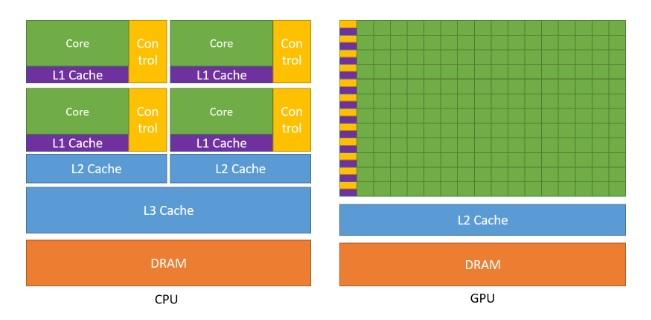
\includegraphics[width=15cm]{Nvidia-CPU-GPU.jpg}				
\caption{Diferencia de arquitectura entre CPU (izquierda) y GPU (derecha) \cite{web}. }
\label{fig:arquitectura-cpu-gpu}
\end{figure}
\noindent

Para generar soluciones que utilicen la paralerización de las tarjetas gráfics Nvidia ha desarrollado CUDA, un lenguaje de programación basado en C, el cual comparte sintaxis en muchos aspectos con este último lenguaje. En CUDA distinguimos dos tipos de procesos, los llevados a cabo en la CPU o 'host' y los ejecutados desde la GPU o 'device', teniendo acceso ambos dispositivos a dos tipos de memoria, global y constante. En la figura \ref{fig:arquitectura-cpu-gpu} se muestra al estructura del device y cómo ambos comparten memoria. Para identificar el lugar de ejecución de cada función cuda ha nombrado como \_\_host\_\_ a las aplicaciones ejecutadas en CPU y \_\_global\_\_ a las ejecutadas en GPU.

Cada tarjeta gráfica tiene un número determinado de hilos (Threads) los cuales pueden realizar un cálculo concreto, simultaneamente, cuando son llamados por una función global (desde el device). Para realizar esta llamada CUDA ha dividido los hilos en bloques y mallas como se puede ver en la figura (1), donde se muestra una malla de dos bloques y dos hilos e cada bloque, siendo 4 los hilos totales.

\begin{figure}[h]
\centering
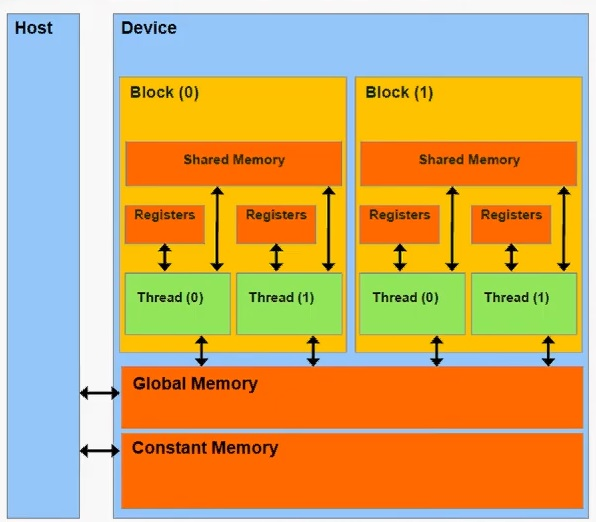
\includegraphics[width=10 cm]{Nvidia-Device_Structure.jpg}				
\caption{Estructura del Host (Documentación de Nvidia [3]). }
\end{figure}
\noindent

En el algoritmo, desde el host se seleccionan el número de hilos a utilizar teniendo en cuenta las limitaciones de hilos por bloques y bloques por mallas de la tarjeta gráfica que se esté utilizando y desde la función global (en el device) se determinan las operaciones a realizar por cada hilo. 

Dadas las variables a utilizar, hilos, bloques y mallas, es necesario identificar el hilo que se quiere utilizar para ejecutar el cálculo. Conceptualmente podemos ver una malla como una matriz, dividida por bloques e hilos dentro de estos bloques como se muestra en la figura (3). En ella se muestra una malla compuesta por 60 hilos, dividida por 4 bloques de 15 hilos cada uno.

\begin{figure}[h]
\centering
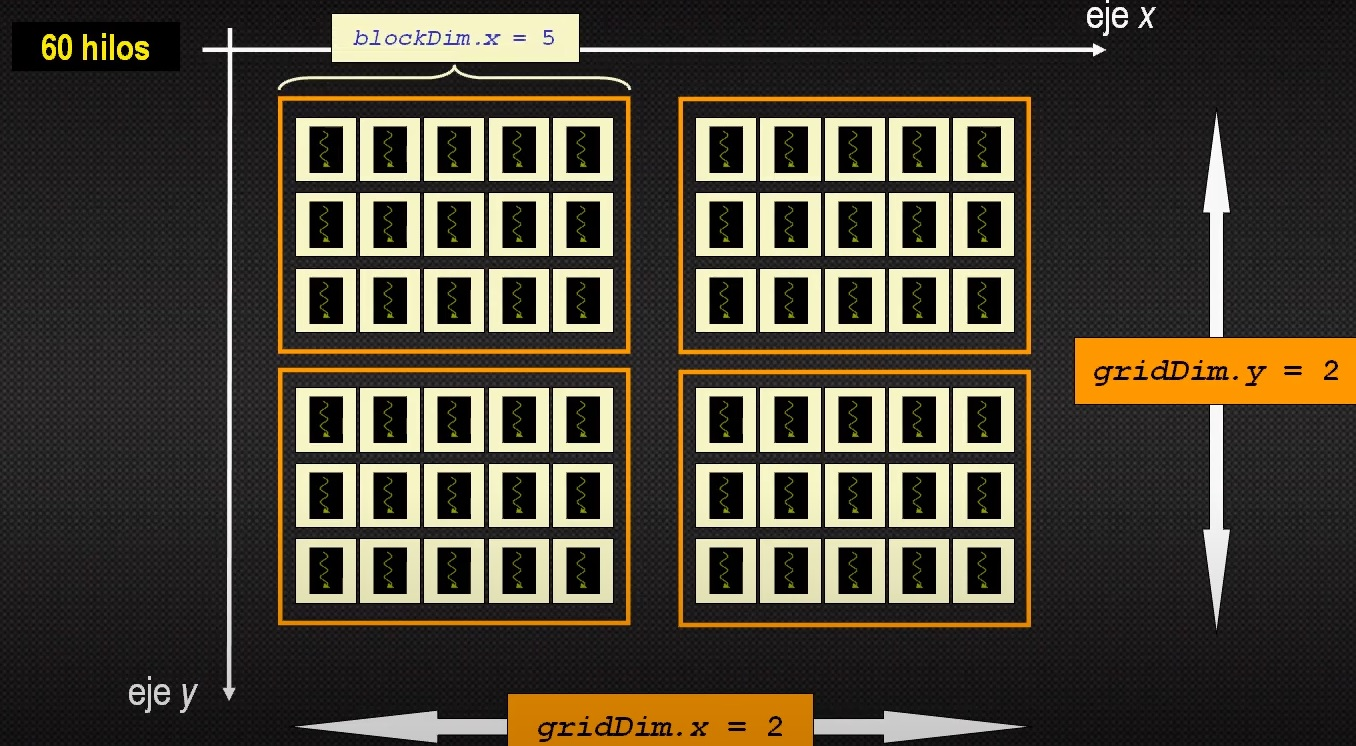
\includegraphics[width=10 cm]{Nvidia_Topologia_virtual.jpg}				
\caption{Topología dentro de hilos, bloques y mallas (Documentación de Nvidia [3]) }
\label{fig:topologia-hilos}
\end{figure}
\noindent

No obstante, la división que hace CUDA de los hilos es lineal como se muestra en la figura \ref{fig:topologia-hilos}. En ella podemos ver separados por franjas claras y oscuras el paso de un bloque a otro. De modo que, para poder identificar un hilo podemos concebir la malla como una matriz donde las filas determinan el bloque y las columnas los hilos. Así, se distingue unívocamente cada hilo multiplicando las columnas totales por el número del bloque donde está el hilo y sumandole la posición que ocupa en el.

\begin{figure}[h]
\centering
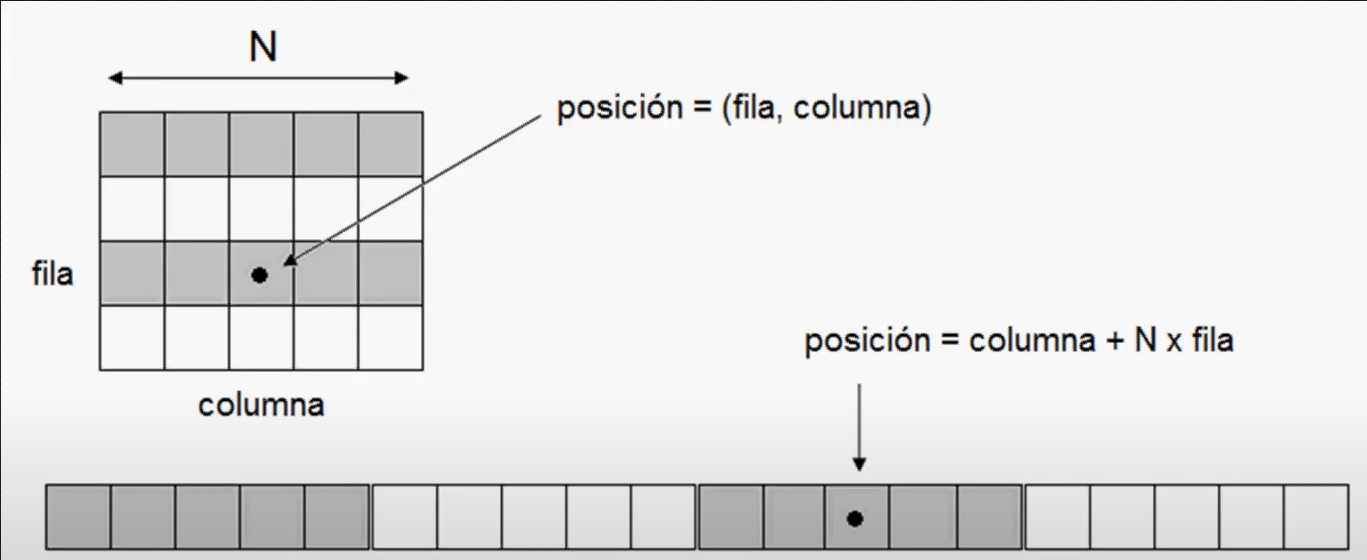
\includegraphics[width=10 cm]{Nvidia_Posicion_hilo.jpg}				
\caption{Identificación de hilo dentro de una malla.}
\end{figure}
\noindent

Esta identificación se lleva a cabo en los algoritmos utilizados en este TFG, denotando las filas y las columnas como 'fil' y 'col' respectivamente, utilizando las palabras reservadas que proporciona CUDA para identificar cada hilo, bloque y malla.

Es necesario resaltar la necesidad de seleccionar la cantidad de hilos y bloques acorde a la capidad de la gráfica y las necesidades del problema. En específico, para la resolución de las ecuaciones de Maxwell en dos dimensiones para un mallado de un millón de puntos, dividido en 1000 posiciones en la dimensión x y 1000 posiciones en la dimensión y, con la gráfica utilizada en este TFG (la cual perrmite 1024 hilos por bloque), es necesario utilizar un mínimo de 977 bloques de 1024 hilos cada uno.

\newpage

\section{Implementación}

A continuación se expone la implementación de las ecuaciones (2.21-2.24) usando CUDA, donde se han desarrollado dos algoritmos, uno usando el poder secuencial de la CPU y otro utilizando la capacidad de paralelización de la GPU. 

En la figura (5) se muestra la implementación en el host, donde se hace uso de varios bucles para realizar el calculo secuencial posición a posición. Dada la reserva de memoria de los punteros en el host, los cuales son vectores aunque se quiera trabajar con matrices, para ver con mas claridad la similitud, se identifica cada posición como se ha expuso en el apartado (1.2).

\begin{verbatim}
	__host__ void check_CUDA_Error(const char* mensaje)
	{
		cudaError_t error;
		cudaDeviceSynchronize();
		error = cudaGetLastError();
		if (error != cudaSuccess)
		{
			printf("ERROR %d: %s (%s)\n", error, cudaGetErrorString(error), mensaje);
            printf("\npulsa INTRO para finalizar...");
            fflush(stdin);
        	char tecla = getchar();
			exit(-1);
		}
	}
\end{verbatim}

%\begin{figure}[h]
%\centering
%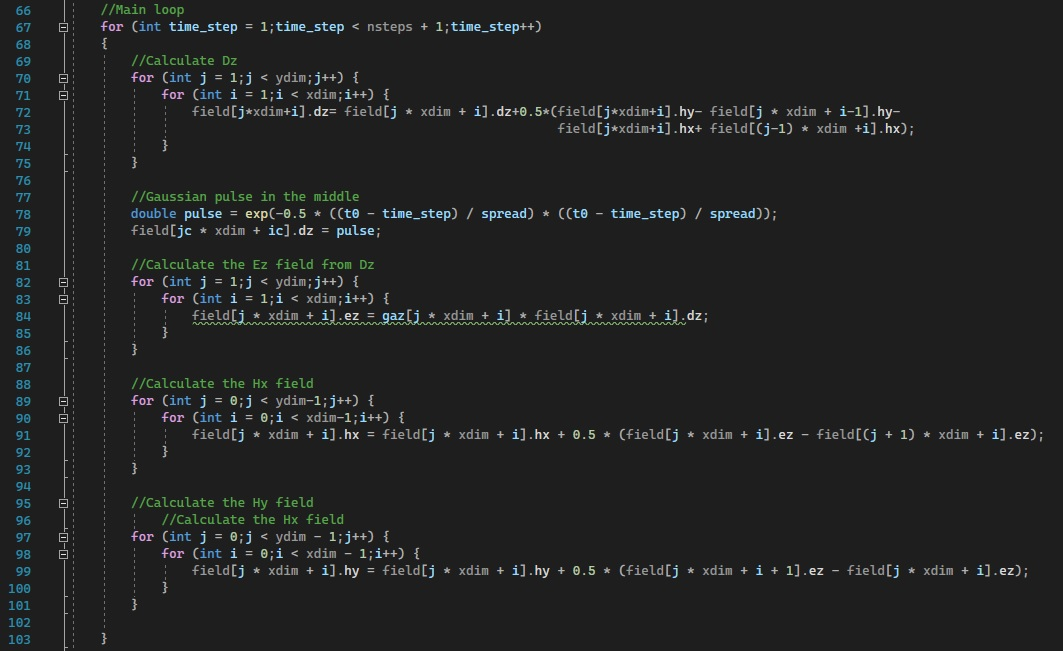
\includegraphics[width=15cm]{FD2D_Host_loop.jpg}				
%\caption{Implementación de las ecuaciones (2.21-2.24) para el cálculo de los campos en la CPU }
%\end{figure}
%\noindent

A diferencia del algoritmo anterior, en la figura (6) se muestra la implementación de las ecuaciones para su cálculo de forma paralela en el device, donde se especifica en los vectores que realicen los cálculos hilo a hilo.

\begin{figure}[h]
\centering
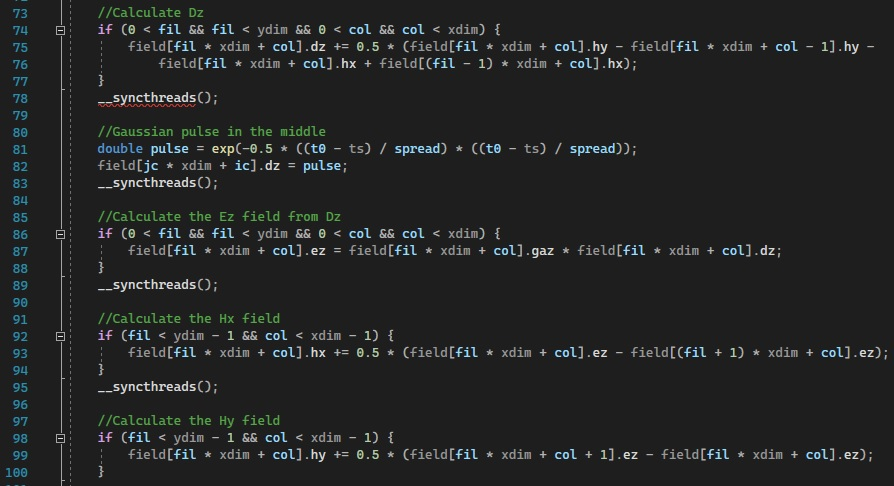
\includegraphics[width=15cm]{FD2D_Kernel_loop.jpg}				
\caption{Implementación de las ecuaciones (2.21-2.24) para el cálculo de los campos en la GPU }
\end{figure}
\noindent




\newpage



\section{Resultados}

\newpage




\section{Conclusiones}



% Referencias %%%%%%%%%%%%%%%%%%%%%%%%%%%%%%%%%%%%%%%%%%%%%%%%%%%%%%%%%%%%%%%%%
\newpage

\addcontentsline{toc}{section}{Referencias} % Elige según idioma
%\addcontentsline{toc}{section}{References} % Elige según idioma

\begin{thebibliography}{100}

\bibitem{Houle2020}
  Jennifer E~Houle and Dennis M~Sullivan, \\
  {\em Electromagnetic simulation using the FDTD method with Python}, \\
  IEEE PRESS WILEY, 2020.
  
\bibitem{Taflove2005}
Allen Taflove and Susan C~Hagness, \\
{\em Computational electrodynamics. The Finite-Difference Time-Domain Method}, \\
ARTECH HOUSE, 2005.

\bibitem{web}
 Nvidia documentation, \\
 \href{https://docs.nvidia.com/cuda/cuda-c-programming-guide/index.html}{https://docs.nvidia.com/cuda/cuda-c-programming-guide/index.html}





 
\end{thebibliography}

\end{document}
